\documentclass[a4paper,12pt]{article}
\usepackage[english]{babel}
\usepackage{setspace}
\usepackage[backend=bibtex, style=chicago-authordate]{biblatex}
\usepackage{graphicx} %for graphics
\graphicspath{ {/home/heidi/Gradu2_0/Images/} }
\addbibresource{mastersthesis.bib}


\begin{document}
\section{Method}
- computer aided network analysis <- distinction between 'verkostotutkimus' mentioned in Juuso Marttila's thesis. 
Quite a few textbooks have been written on network analysis.

\subsection{Defining the network}
Network analysis is based on the mathematical graph theory. A graph is a representation of the network. Graph includes nodes and edges.

\begin{figure}[h]
	\caption{A sample from the graph} 
	\centering
	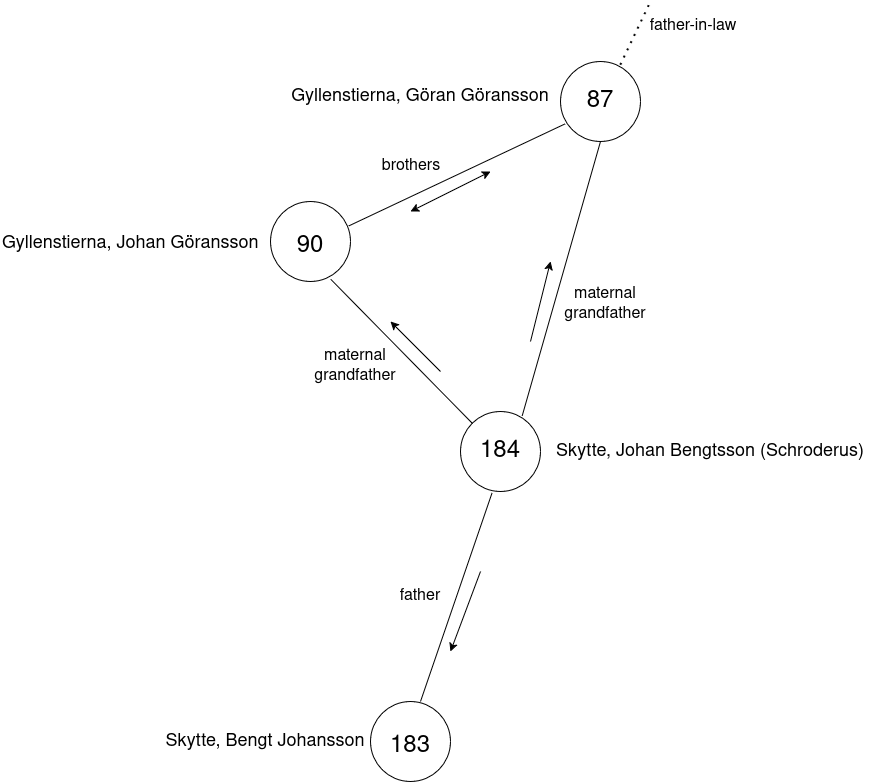
\includegraphics[scale=0.25]{example_network.drawio.png}
	\centering	
\end{figure}
In this context the graph's nodes depict individual councilors with the input of name and id number. Correspondingly the edges represent the kinships between two nodes. For instance, in Figure 1 we can see that Johan Bengtsson (Schroderus) Skytte (id 184) is Bengt Johansson Skytte's (id 183) father and a maternal grandfather for Johan Göransson Gyllenstierna (id 90) and Göran Göransson Gyllenstierna (id 87). Johan Göransson and Göran Göransson are brothers, however, their father is not mentioned in the dataset. Göran Göransson also has further links in the network. \footfullcite{councilorsDS} 

\subsection{Implementation of the network analysis}
The data processing and analysis is conducted with a combination of Python programming language and Gephi software. Python is used for extracting the data from the Councilors-dataset and formulating it in the right format: readable for Gephi. The actual network analysis, visualization and calculating statistics, is performed with Gephi. 

Python is a programming language commonly used in scientific work.
On my opinion simple syntax, easy to implement smaller tasks such as data processing. Readable, widely used therefore makes the work replicable. 

As graphs are structures commonly used in programming, it would have been possible to conduct the actual network analysis using tools provided by Python, yet, Gephi software provides a visual user interface and more intuitive tools for the manipulation of the graph.

Gephi is ...

Both of these tools are also open source and free to download.

All scripts written for this work available on github.

How the data was processed, removing the end of the dataset with calc tools TODO add also to the source section about the end
the test run and "first look " pdf

Problems: we don't have data about the women

\end{document}
